\documentclass[a4paper,man,floatsintext,longtable,noextraspace,12pt]{apa6}

\usepackage[english]{babel}
\usepackage[utf8x]{inputenc}
\usepackage{amsmath}
\usepackage{graphicx}
\usepackage[colorinlistoftodos]{todonotes}
\usepackage{hyperref}

\usepackage{booktabs}
\usepackage{longtable}
\usepackage{array}
\usepackage{multirow}
\usepackage{wrapfig}
\usepackage{float}
\usepackage{colortbl}
\usepackage{pdflscape}
\usepackage{tabu}
\usepackage{threeparttable}
\usepackage{threeparttablex}
\usepackage[normalem]{ulem}
\usepackage{makecell}
\usepackage{xcolor}
% make captions italic

% number lines
% \usepackage{lineno}
% \linenumbers
            
% bibliography
\newlength{\cslhangindent}
\setlength{\cslhangindent}{1.5em}
\newenvironment{CSLReferences}%
  {}%
  {\par}

% tightlist
\providecommand{\tightlist}{%
  \setlength{\itemsep}{0pt}\setlength{\parskip}{0pt}}

\title{\textbf{How open are hybrid journals included in transformative agreements?}}
\shorttitle{Hybrid OA}
\author{Najko Jahn}
\affiliation{Göttingen State and University Library, University of Göttingen\\
Platz der Göttinger Sieben 1, 37073 Göttingen, Germany\\
najko.jahn@sub.uni-goettingen.de
}

%\authornote{Correspondence concerning this article should be addressed to Najko Jahn}

\abstract{}

\begin{document}
\maketitle

% QSS wants numbered sections
%\setcounter{secnumdepth}{2}

\hypertarget{introduction}{%
\section{Introduction}\label{introduction}}

For over two decades, hybrid open access journal publishing, which makes
some articles openly available while others remain behind a paywall, has
been discussed as a means for transitioning the subscription system to
full open access (Prosser, 2003). The idea was that when journals
increasingly publish open access articles, they could reduce revenues
from subscriptions, while libraries and funders could change their
funding models and shift expenditures from subscription to open access.
However, initial approaches, mainly based on publication fees, also
called article processing charges (APCs), did not contribute
substantially to a large open access uptake. In 2009, Springer reported
open access to 1\% of articles in hybrid journals (Dallmeier-Tiessen et
al., 2010). Other studies also recorded a low uptake. In 2011, only
1-2\% of articles were open access (Björk, 2012), growing to around 4\%
between 2011 and 2013 (Laakso \& Björk, 2016).

With the introduction of central funding mechanisms for publication fees
in some European countries since 2012, an increase in hybrid open access
could be observed (Björk, 2017; Huang et al., 2020; Jubb et al., 2017;
Piwowar et al., 2018). For example, studying university output,
Robinson-Garcia et al. (2020) estimated a median uptake of 7.1\% in the
period 2014-2017. In particular, British (17\%), Austrian (15\%) and
Dutch (13\%) universities contributed to this trend. However, this shift
in funding policy towards hybrid open access also added to the overall
cost of publishing, which includes subscription spending and the
administrative efforts required to handle payments (Pinfield et al.,
2016). Moreover, established large commercial publishers, which already
dominated the publishing market (Larivière et al., 2015),
disproportionately benefited from hybrid open access funding in
comparison to full open access publishers (Butler et al., 2023; Jahn \&
Tullney, 2016; Shu \& Larivière, 2023).

As a consequence, libraries and their consortia began to develop
licensing strategies aimed at avoiding such `double dipping' scenarios,
in which well-established commercial publishers gain twice from reading
and open access publishing, as well as to increase publisher-provided
immediate open access (Björk \& Solomon, 2014; Schimmer et al., 2015).
These considerations resulted into transformative agreements, which
cover a broad range of contracts between library consortia and
publishers from mid-2010s onwards where institutional spending for
subscriptions and open access publishing are considered together
(Borrego et al., 2020; Hinchliffe, 2019). Transformative agreements seek
to control costs while allowing a transitional phase for publishing more
open access articles. Similar to big deals, transformative agreements
mainly bundle hybrid and subscription-only journals from commercial
publishers, but aim at a higher degree of transparency than previous big
deals, where contracts including payments were confidential (Bergstrom
et al., 2014).

The introduction of transformative agreements aligns with funding policy
changes, such as the decision made by the cOAlition S, a consortium of
national funders including the European Commission, to no longer provide
financial support for individual publication fees when publishing in
hybrid journals. According ot its Plan S launched in 2018, the cOAlition
S funders only accept hybrid open access through transformative
agreements ``during a transition period that should be as short as
possible'' (Schiltz, 2018). Specifically, they agreed to support hybrid
open access only through transformative agreements from 2021, until the
end of 2024. Notably, the German Research Foundation (DFG), despite not
being part of cOAlition S, has also extended its financial support for
hybrid open access through transformative agreements (Mittermaier,
2021). Previously, the DFG only provided funding for full open access
journals (Jahn \& Tullney, 2016).

By the end of 2023, many transformative agreements were implemented, but
interim outcomes are mixed. The ESAC Transformative Agreement
Registry\footnote{\url{https://esac-initiative.org/about/transformative-agreements/agreement-registry/}},
the largest source of disclosure, recorded more than 800 transformative
agreements, resulting in up to 900.000 open access articles published in
both full open access and hybrid journals according to the accompanying
ESAC Market Watch\footnote{\url{https://esac-initiative.org/market-watch/}}.
Library consortia reported increased open access volume, streamlined
payment and monitoring procedures, as well as extensive utilization of
open access options by the researchers they serve (Marques \& Stone,
2020; Parmhed \& Säll, 2023; Pinhasi et al., 2020). The ongoing
standardisation of transformative agreements contributed to improved
transparency in terms of contracts and publisher-provided article
metadata (Marques et al., 2019; Pinhasi et al., 2021). However, with the
growing trend toward transformative agreements, continued reliance on
big deals is perceived as problematic, because it perpetuate market
concentration (Butler et al., 2023; Shu \& Larivière, 2023). Whether
transformative agreements lead to reduced pricing remains uncertain
(Borrego, 2023) and a substantial transition of hybrid journals towards
full open access could not be observed (Matthias et al., 2019; Momeni et
al., 2021). The focus on large commercial publishers might also increase
inequality, because transformative agreements focus on pay to publish
open access mainly targets institutions from high-income countries,
furthering a questionable journal prestige culture (\textbf{budapest?}).
Besides, an editorial-board resignation raised concerns that publishers'
desire to maximize journal publication volume ``without regard to
quality'' is a consequence of transformative agreements (Rasmussen,
2023).

The controversies surrounding hybrid open access and transformative
agreements have led to varying policy conclusions. For instance, the
Association of Swedish Higher Education Institutions (Sveriges
universitets- och högskoleförbund, SUHF) recommended to only support
agreements for publishing in full open access journals \footnote{\url{https://www.su.se/english/news/open-access-need-to-move-away-from-transformative-agreements-1.683787}}.
Likewise, most cOAlition S funders will discontinue financial support
for transformative agreements by the end of 2024 (Liverpool, 2023). The
consortium also removed most hybrid journals from its Transformative
Journal program in 2023 due to publishers' failure to meet self-defined
open access growth targets (Brainard, 2023). In contrast, the German
DEAL consortium signed a five-year transformative agreement with
Elsevier starting in 2024, while also renewing its contracts with
Springer Nature and Wiley until the end of 2028.

Despite these controversies around transformative agreements as a means
of transitioning journal publishing to full open access, there is
limited evidence available on the adoption of open access in hybrid
journals, and the extent to which this uptake can be attributed to
transformative agreements. Previous studies have focused on specific
countries (Haucap et al., 2021; Huang et al., 2020; Pölönen et al.,
2020; Taubert et al., 2023; Wenaas, 2022) or publisher portfolios
(Bakker et al., 2024; Fraser et al., 2023; Jahn et al., 2022; Momeni et
al., 2023; Pieper \& Broschinski, 2018), while large-scale studies
relied on self-reported agreement data (Moskovkin et al., 2022), or used
APC pricing lists (Shu \& Larivière, 2023). Particularly, data
availability is a limiting factor when studying the impact of
transformative agreements (Bakker et al., 2024), because bibliometric
databases, even though many allow the retrieval of open access articles
in hybrid journals, do not directly attribute them to specific
transformative agreements.

The present study aims to address these limitations by combining
multiple openly available data sources to determine the open access
uptake in hybrid journals, while distinguishing between open access
through transformative agreements and other means. With this novel and
open approach, this the first large-scale analysis aims to answer the
following questions:

\begin{itemize}
\tightlist
\item
  What was the number and proportion of open access articles in hybrid
  journals in transformative agreements between 2018 and 2022?
\item
  To what extent did institutions with a transformation agreement
  contribute to the adoption of open access in hybrid journals?
\end{itemize}

For both of these research questions, this study will analyse the
variability by publisher, journal subject, and country.

\hypertarget{methods}{%
\section{Methods}\label{methods}}

This study combines data from multiple publicly available data sources
as diagrammatically shown in Figure \ref{fig:data_workflow}. Initially,
transformative agreement data retrieved from the cOAlition S Journal
Checker Tool\footnote{\url{https://www.coalition-s.org/blog/enabling-accurate-results-within-the-journal-checker-tool/}}
provided information about journal portfolios and participating
institutions. After identification of hybrid journals by excluding full
open access journals, Crossref served as the primary data source for
article-level metadata including Creative Commons (CC) license
information to indicate open access availability on publisher websites.
To determine open access articles published through transformative
agreements, first author affiliations from OpenAlex (Priem et al., 2022)
were subsequently linked to eligible institutions according to the
transformative agreement data. In the following, these steps are
described in more detail.

\begin{figure}[ht!]

{\centering 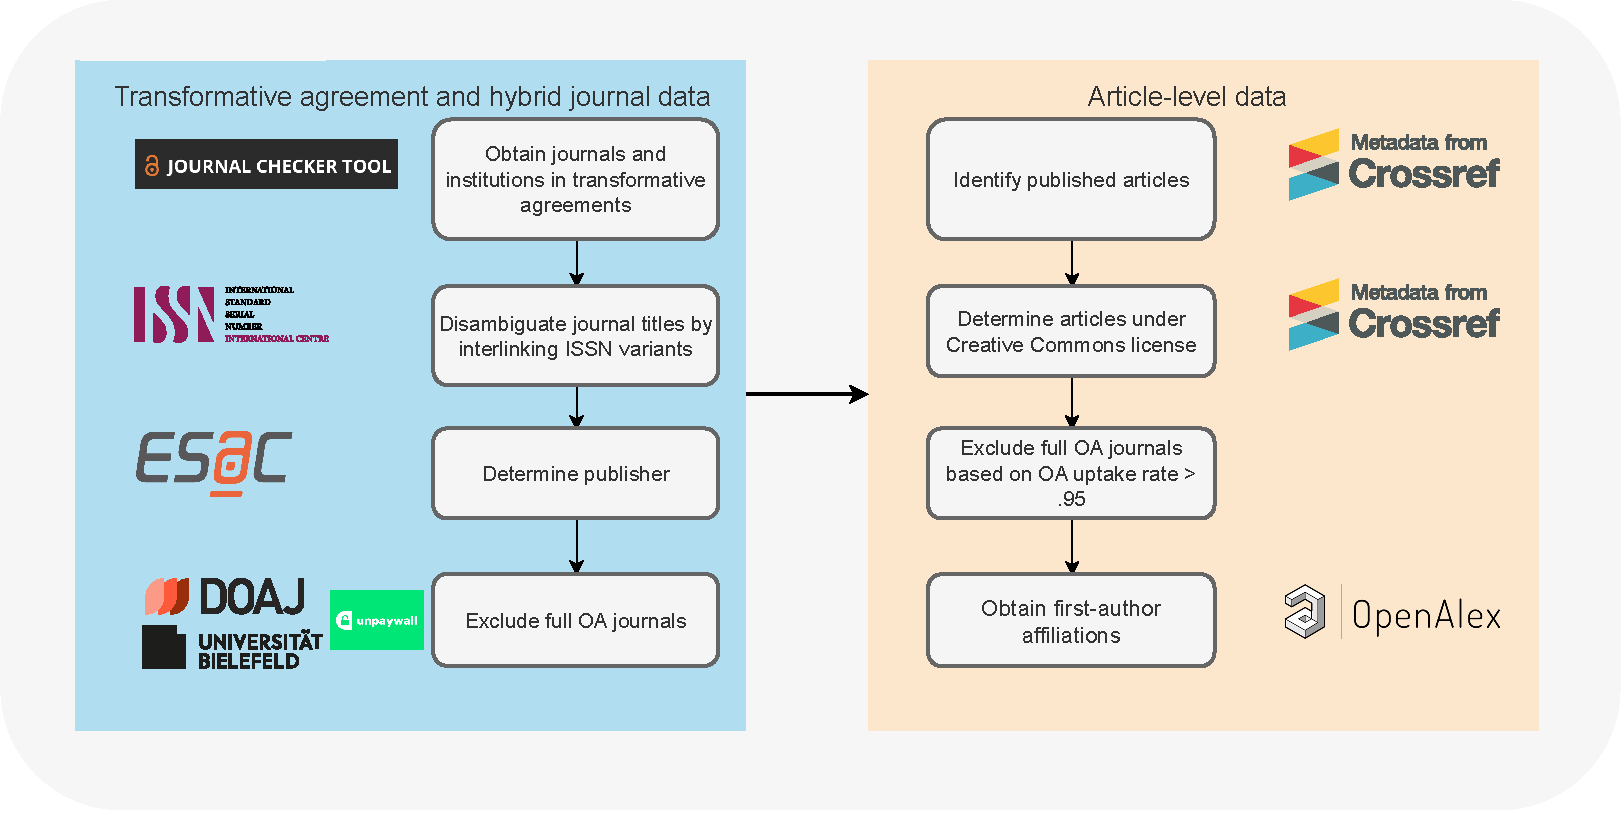
\includegraphics[width=0.99\linewidth,]{data_collection_workflow} 

}

\caption{Data collection workflow}\label{fig:data_workflow}
\end{figure}

\hypertarget{transformative-agreement-and-hybrid-journal-data}{%
\subsection{Transformative agreement and hybrid journal
data}\label{transformative-agreement-and-hybrid-journal-data}}

Data gathering started with obtaining journals included in
transformative agreements from the publicly available Transformative
Agreement Data dump\footnote{\url{https://journalcheckertool.org/transformative-agreements/}}
used by the cOAlition S Journal Checker Tool.\footnote{\url{https://www.coalition-s.org/blog/enabling-accurate-results-within-the-journal-checker-tool/}}
The dump consists of multiple online Google spreadsheets where each data
file represents one agreement listed in the ESAC Transformative
Agreement Registry.\footnote{\url{https://esac-initiative.org/about/transformative-agreements/agreement-registry/}}
From the retrieved spreadsheet files, journals and institutions involved
per agreement were obtained.

A limitation of using the Journal Checker Tool and its underlying
publicly available data dump to study the development of transformative
agreements over time is that expired transformative agreements are
constantly removed. To address this, four different snapshots were
safeguarded and combined for this study: self-archived versions from
July 2021, July 2022, and May 2023, as well as the most current dump
downloaded on 11 December 2023. This ensured that transformative
agreements, which ended from 2021 onwards, were included, representing
the majority of transformative agreements. Overall, the four combined
Transformative Agreement Data dumps used in this study contained 729 out
of 869 agreements listed in the ESAC registry by December 2023.

The Transformative Agreement Data dumps link agreements to journals
represented by journal names and ISSN. After mapping ISSN variants to
the corresponding linking ISSN (ISSN-L) as provided by the ISSN
International Centre, journals were associated to publishers using the
ESAC ID, a unique identifier for transformative agreements in the ESAC
Transformative Agreement Registry. Furthermore, journal subjects
according to the All Science Journal Classification code (ASJC) were
added from the Scopus journal source list as of August 2023.

Because transformative agreements can include both full open access and
hybrid journals, the data were complemented with information about a
journal's open access status using multiple sources: the Directory of
Open Access Journals (DOAJ) downloaded on 12 December 2023\footnote{\url{https://doaj.org/csv}},
OpenAlex (November 2023) and the the Bielefeld list of GOLD OA journals
(Bruns et al., 2022). As shown in Figure \ref{fig:method_fig}A,
combining different data sources considerably extended the journal
matching. In total, 3,439 full open access journals were excluded based
on ISSN matching. The overlap between the three data sources was 72\%.
The Gold OA journals dataset alone added 176 journals, while the DOAJ
comprised 10 full open access journals not listed in either of the other
two sources. These full open access journals were mostly launched in
2022.

\hypertarget{article-and-author-metadata}{%
\subsection{Article and author
metadata}\label{article-and-author-metadata}}

After identifying hybrid journals included in transformative agreements,
article metadata was retrieved from the Crossref November 2023 database
snapshot for the five-year period 2018 to 2022 according to the issued
date, representing the earliest known publication date. Because Crossref
metadata lacked information to distinguish between original research
articles including review and other types of journal content, which are
often not covered by transformative agreements (Borrego et al., 2020),
only articles published in regular issues indicated by non-numeric
pagination were included. Furthermore, an expanded version of
Unpaywall's paratext recognition approach was applied to exclude
non-scholarly journal content such as table of contents.

Open access articles in hybrid journals were identified through Creative
Commons (CC) license information in Crossref metadata. License
information relative to the ``accepted manuscript (AM)'' version were
not considered. Crossref was used for open access identification because
transformative agreements workflows generally require publishers to
deliver CC license information to this DOI registration agency (Geschuhn
\& Stone, 2017). Comparing Crossref license coverage with OpenAlex,
which re-uses open access evidence from Unpaywall, a widely used open
access discovery service that also parses journal websites for open
content licenses (Piwowar et al., 2018), highlighted ongoing challenges
to identify hybrid open access (Butler et al., 2023; Jahn et al., 2022;
Martín-Martín et al., 2018; Zhang et al., 2022). Here, 742,369 articles
with CC license were retrieved using Crossref, while 950,260 articles
were tagged as ``hybrid'' according to the OpenAlex November 2023
release, which was used throughout this study. The biggest differences
concerned articles published between 2018 and 2020. In 2022, however,
Crossref and OpenAlex open access numbers only differ slightly (249,511
records using Crossref vs.~255,344 in OpenAlex). Notable difference
could be furthermore observed among some publishers that presumably did
not provide CC license information to Crossref including AIP Publishing,
American Physiological Society, Emerald and the Royal Society. Crossref
license metadata was more complete with regard to articles from the
publisher Wiley and American Chemical Society. Finally, inconsistent
open access status information in previous OpenAlex versions was
observed (Jahn et al., 2023). After reporting it to OpenAlex, according
to the release notes, fixing this issue was still ongoing, which might
also explain part of the discrepancy.

After retrieving article metadata, the publication volume including open
access was calculated per journal. To improve the identification of
hybrid journals, journals with an open access proportion above 95\% were
excluded. This further step allowed to remove additional 241 full open
access journals.

Affiliation metadata about corresponding authors are crucial for the
planning and evaluation of transformative agreements, because they are
considered to be responsible to arrange open access publication (Borrego
et al., 2020; Geschuhn \& Stone, 2017; Schimmer et al., 2015). Here,
country and institutional affiliations were retrieved from OpenAlex.
However, because of low coverage in OpenAlex, this study focused on
first authors and their affiliations instead. First authors typically
contribute most to a paper and are often considered lead author research
papers (Larivière et al., 2016). Related studies therefore assumed first
authors as a proxy to measure to open access payments and the impact of
transformative agreement (Haucap et al., 2021; Shu \& Larivière, 2023;
Zhang et al., 2022). Overall, around 90\% of studied articles had first
author affiliation metadata in OpenAlex, whereas the coverage of
articles with corresponding author information was around 54\%.

To assess the impact of transformative agreements to hybrid open access,
participating institutions from the Transformative Agreement Data dump,
which were crowd-sourced from the agreements and consortia that
successfully negotiated an agreement, were matched with first author
affiliations recorded by OpenAlex using the ROR-ID. The matching also
took into account the duration of an agreement according to the ESAC
registry. Upon inspection, Transformative Agreement Data did not cover
associated institutions comprehensively like university hospitals or
institutes of large research organisations like the Max Planck Society.
To improve the matching, Transformative Agreement Data was automatically
enriched with associated organisations using OpenAlex's institution
entity data.

In total, the compiled data set consists of 8,922,146 articles published
in 12,857 hybrid journals between 2018 and 2022 (see Figure
\ref{fig:method_fig}B). Hybrid journals in transformative agreements
represented 40\% of total global output over the same time period
according to Crossref, while full open access journals recorded 35\%.

\begin{figure}[ht!]

{\centering 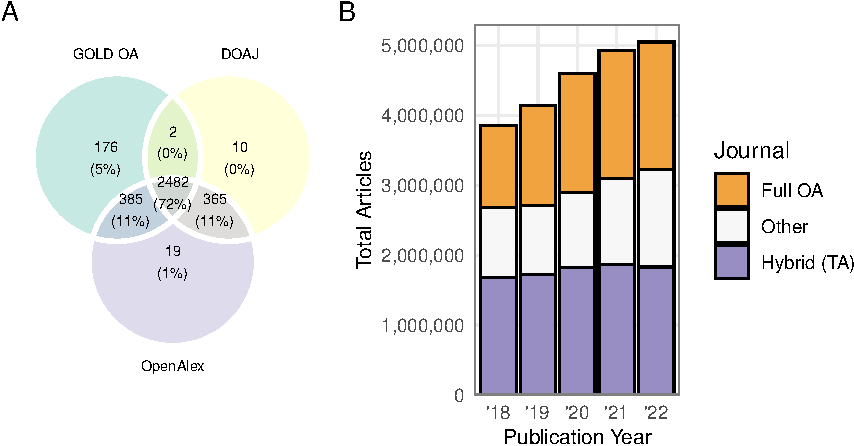
\includegraphics[width=0.99\linewidth,]{fig/method_fig-1} 

}

\caption{Initial data characteristics. (A) Full open access journals included in transformative agreements by evidence source Directory of Open Access Journals (DOAJ), OpenAlex and the Bielefeld GOLD OA list. (B) Number of articles in Crossref by journal types. The blue bars show the overall article volume of hybrid journals in transformative agreements, which were initially included in the study, in comaprision with full open access journals according to OpenAlex. The remainder represents closed access journals not covered by transformative agreements.}\label{fig:method_fig}
\end{figure}

\hypertarget{data-analysis}{%
\subsection{Data Analysis}\label{data-analysis}}

Throughout this mostly automated data gathering and analysis process,
tools from the Tidyverse (Wickham et al., 2019) for the R programming
language (R Core Team, 2020) were used. The resulting data is openly
available through an R data package, hoaddata, version 0.2.91 Following
Marwick et al. (2018), hoaddata contains not only the datasets used in
the data analysis. It also includes code used to compile the data by
connecting it the cloud-based Google Big Query data warehouse, where the
big scholarly data from Crossref, OpenAlex and Unpaywall were imported.
To increase the computational reproducibility, the data aggregation
through hoaddata was automatically carried out using GitHub Actions, a
continuous integration service.

\hypertarget{results}{%
\section{Results}\label{results}}

\hypertarget{overview}{%
\subsection{Overview}\label{overview}}

Between 2018 and 2022, a total of 11,189 out of 12,857 hybrid journals
in transformative agreements published at least one open access article
under a Creative Commons license. During this period, these hybrid
journals provided open access to 742,369 out of 8,146,958 articles,
representing a five-year open access proportion of 9.1\%. Authors who
could make use of transformative agreements at the time of publication
contributed 328,957 open access articles to the total.

\begin{figure}[ht!]

{\centering 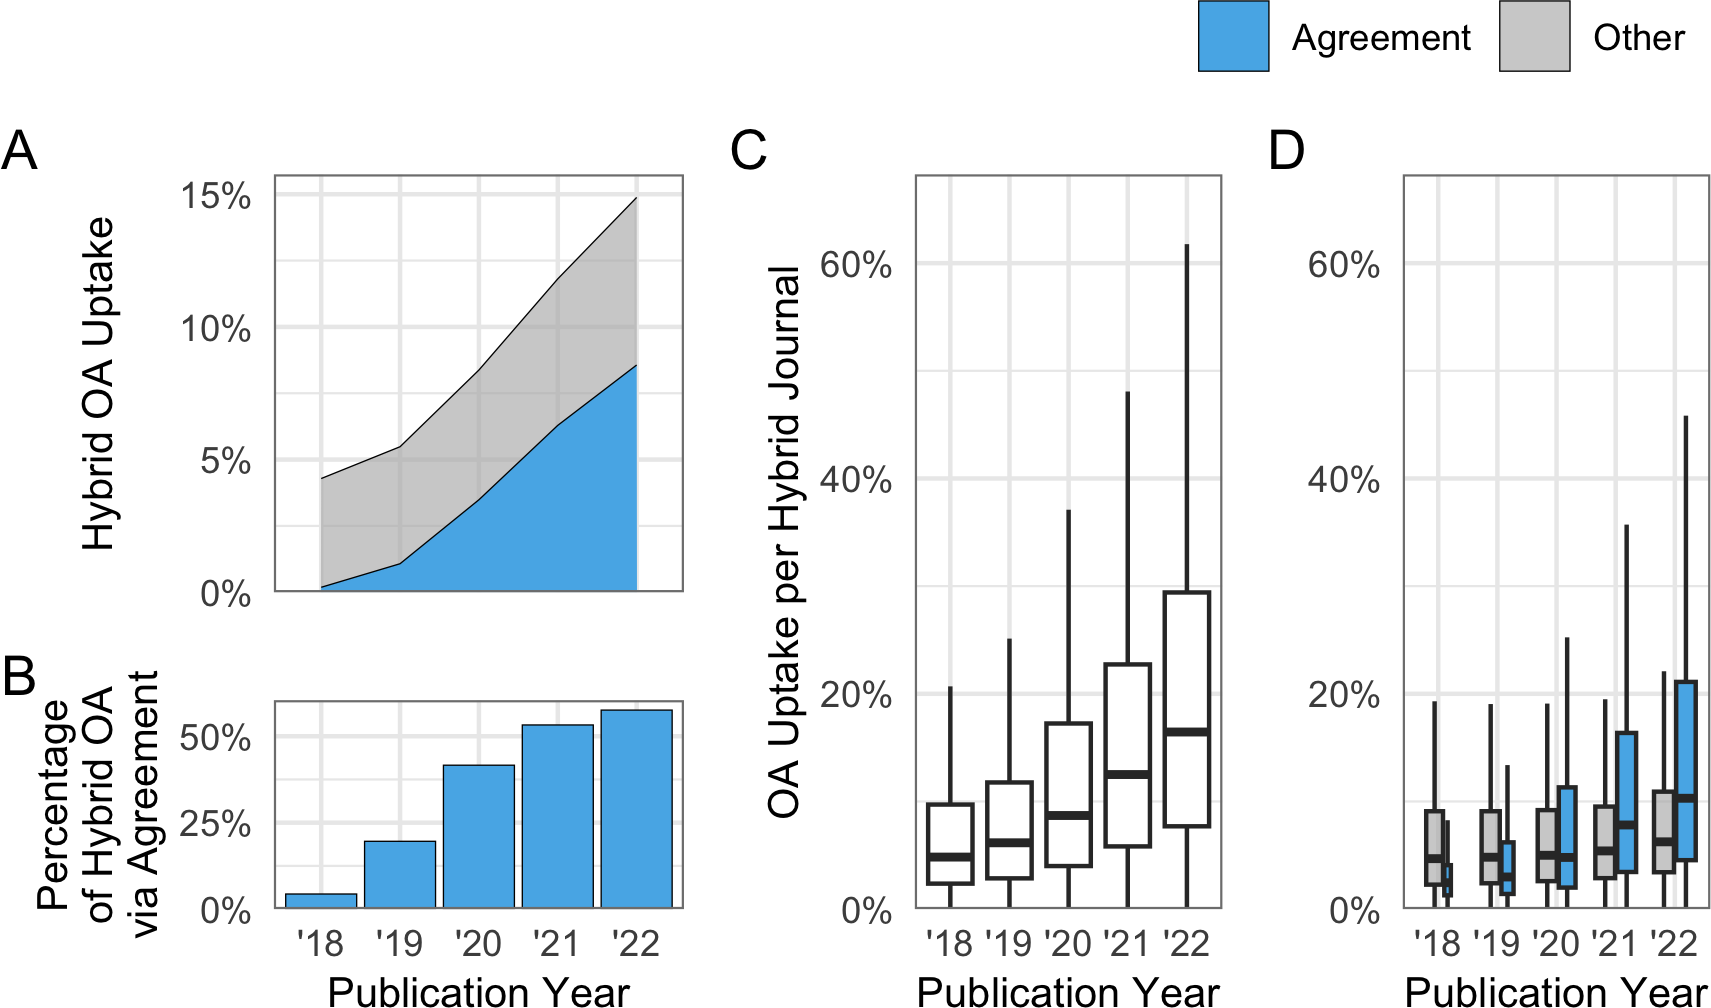
\includegraphics[width=0.99\linewidth,]{fig/results_overview-1} 

}

\caption{Relative growth of open access in hybrid journals in transformative agreements between 2018 and 2022 per publication year. The blue areas represent open access through transformative agreements, the grey areas depict open access articles where no link to an agreement could be established. (A) Proportion of open access articles in hybrid journals per year. (B) Percentage of hybrid open access via agreements per year. Boxplots show the proportion of open access articles by individual hybrid journals (C) and individual open access uptake rates by individual hybrid journals and open access funding (D) per publication year. The individual outliers are not shown. Note that data on transformative agreements ending before June 2021 were not available for this study.}\label{fig:results_overview}
\end{figure}

Figure \ref{fig:results_overview}A shows a moderate growth in the
proportion of open access articles in hybrid journals, comparing the
overall open access uptake and the impact of transformative agreements
on this trend. Over the five-years period from 2018 to 2022, open access
increased from 4.3\% (n = 65,486) to 15\% (n = 249,511). At the same
time, the total article volume of the investigated journals grew from
1,528,051 in 2018 to 1,676,928 in 2022.

Figure \ref{fig:results_overview}B highlights that the majority of
hybrid open access was made available through transformative agreements
in 2021 and 2022, contributing 58\% of the total open access article
volume in 2022. However, there was also a notable growth in open access
provision through other means, most likely publication fees being not
invoiced through transformative agreements, which increased from 4.1\%
(n = 62,625) in 2018 to 6.3\% (n = 105,896).

Figure \ref{fig:results_overview}C depicts the substantial variations
among the hybrid journals included in transformative agreements in terms
of open access uptake. Although the median generally follows the trend
shown in Figure \ref{fig:results_overview}A, the farther stretch of
upper quartiles and whiskers over the years illustrates that an
increasing number of journals published an above-average proportion of
open access articles. In 2022, 25\% of hybrid journals (n = 2,576) had
an open access uptake of 29\%, and 6.6\% of journals (n = 744) provided
the majority of their articles under a Creative Commons license in the
same year. These journals were, on average, smaller (M = 75, SD = 186)
than those with an open access share below 50\% (M = 164, SD = 347).

When comparing the impact of open access trough transformative
agreements across journals, it shows that for many journals these
agreements substantially contributed to the growth of open access over
the years (Figure \ref{fig:results_overview}D). Despite the rise in
transformative agreements, it is worth noting that other means of
publishing open access remained common across the investiagted hybrid
journals. In total, 9,153 journals published open access articles from
authors affiliated with institutions without transformative agreements
in place, while 8,780 journals published at least one open access
article through a transformative agreement in the same year.

\hypertarget{publishing-market}{%
\subsection{Publishing market}\label{publishing-market}}

Analysing hybrid open access across publishers between 2018 and 2022
reveals a large market concentration. Although 48 publishers offered
transformative agreements, the big three commercial publishers Elsevier,
Springer Nature, and Wiley accounted for 49\% of total article volume
published (see Table \ref{tab:publisher_league_table}). Together, they
published 500,878 or 66\% of open access articles in hybrid journals.
Elsevier, Springer Nature, and Wiley made 243,891 articles open access
in hybrid journals through transformative agreements, resulting in an
even larger market share of 74\%.

\begin{table}[H]

\caption{\label{tab:publisher_league_table}Hybrid open access through transformative agreements market shares 2018-2022}
\centering
\begin{tabular}[t]{lrlrlrlrl}
\toprule
\multicolumn{1}{c}{ } & \multicolumn{2}{c}{Hybrid journals} & \multicolumn{2}{c}{Articles} & \multicolumn{2}{c}{OA articles} & \multicolumn{2}{c}{TA OA articles} \\
\cmidrule(l{3pt}r{3pt}){2-3} \cmidrule(l{3pt}r{3pt}){4-5} \cmidrule(l{3pt}r{3pt}){6-7} \cmidrule(l{3pt}r{3pt}){8-9}
Publisher & Total & \% & Total & \% & Total & \% & Total & \%\\
\midrule
Elsevier & 1,936 & 17 & 2,770,826 & 33.8 & 172,723 & 22.9 & 60,440 & 18.3\\
Springer Nature & 2,274 & 20 & 1,330,430 & 16.2 & 175,432 & 23.3 & 100,008 & 30.3\\
Wiley & 1,410 & 12.4 & 1,043,052 & 12.7 & 152,723 & 20.3 & 83,443 & 25.3\\
Other & 5,767 & 50.6 & 3,061,337 & 37.3 & 252,523 & 33.5 & 86,294 & 26.1\\
\bottomrule
\end{tabular}
\end{table}

However, there are notable differences among the three big publishers.
Although Elsevier published the largest volume of articles (n =
2,770,826, 34\%), it recorded a comparable low number of open access
articles, including those that can be associated with transformative
agreements. In contrast, Springer Nature and Wiley provided open access
to a larger proportion of their articles (13\% of Springer Nature
articles and 15\% of Wiley articles were open acccess), leading to
higher open access market shares (23\% Springer Nature resp. 23\%
Wiley). This difference between Elsevier on the one hand and Springer
Nature and Wiley on the other can be attributed to transformative
agreements, as the latter made the majority of their open access
articles available through such deals (Springer Nature 57\% resp. Wiley
55\%).

Figure \ref{fig:publisher_figure} takes a closer look into the growth of
hybrid open access across publishers by year with a focus on open
articles enabled by transformative agreements. Although all publishers
show a general long-term trend towards transformative agreements, Figure
\ref{fig:publisher_figure}A and B indicate that, in particular, Wiley
experienced a substantial increase in its open access share from 5.9\%
(n = 11,628) in 2018 to 26\% (n = 53,503) in 2022, representing an
4.5-fold increase. In contrast, Elsevier's hybrid journals demonstrated
a more modest increase, from 3.3\% (n = 16,872) in 2018 to 10\% (n =
60,821) in 2022, which is a relatively low open access share compared to
the general trend. In 2018, Springer Nature had the largest open access
proportion among the three publishers of 8.4\% (n = 19,701), but
experienced a relatively slower growth, resulting in 18\% (n = 52,616)
of articles being open access in Springer Nature hybrid journals in
2022.

\begin{figure}[ht!]

{\centering 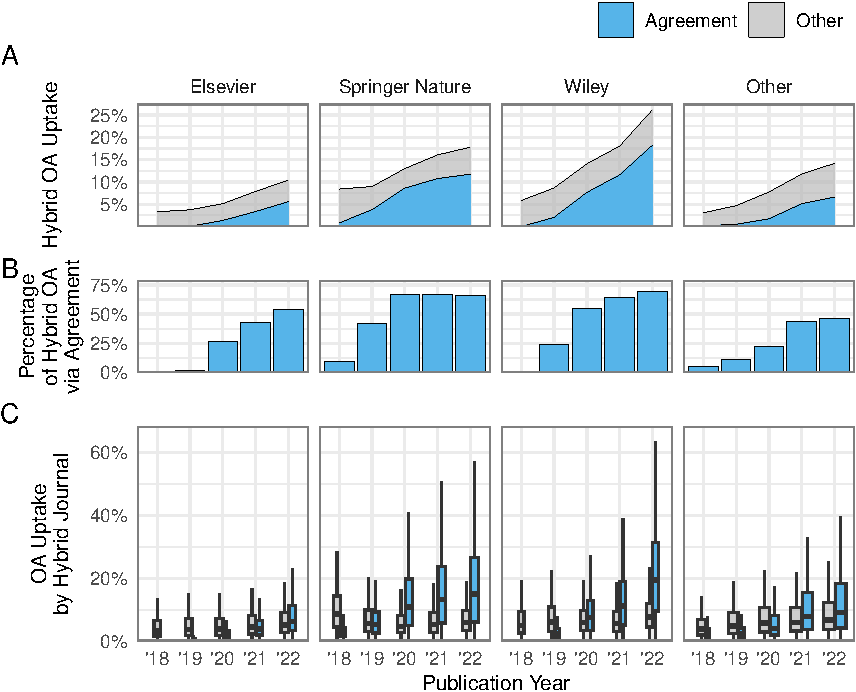
\includegraphics[width=0.99\linewidth,]{fig/publisher_figure-1} 

}

\caption{Developement of open access in hybrid journals included in transformative agreements between 2018 and 2022 by publishers. The blue areas represent open access through transformative agreements, the grey areas depict open access articles where no link to an agreement could be established. (A) Proportion of open access articles in hybrid journals per year and publisher. (B) Percentage of hybrid open access via agreements per year and publisher. Boxplots (C) show individual open access uptake rates by individual hybrid journals and open access funding per publication year and publisher. The individual outliers are not shown. Note that data on transformative agreements ending before June 2021 were not available for this study.}\label{fig:publisher_figure}
\end{figure}

The varying degrees of adoption of open access across the three major
publishers can be attributed to distinct approaches to transformative
agreements. Springer Nature, for example, began in 2015 offering
selected consortia, such as the Max Planck Society, the Swedish Bibsam
consortium, and the Finnish FinELib consortium, open access agreements
for its hybrid journal portfolio under the name Springer
Compact\footnote{\url{https://web.archive.org/web/20180414062853id_/http://www.liber2015.org.uk/wp-content/uploads/2015/03/Springer-Compact.pdf}}.
However, these agreements were not included in the data as they
concluded prior to the start of the transformative agreement data
collection in June 2021. Nonetheless, the results demonstrate the
importance of agreements for Springer Nature's hybrid open access
business over the past five years (Figure 2B). In 2022, 66\% (n =
34,725) of open access in Springer Nature hybrid journals were enabled
through transformative agreements. In the same year, 70\% (n = 37,316)
of Wiley's open access articles could be linked to transformative
agreements in 2022. In contrast, Elsevier published fewer than half of
its open access articles through transformative agreements (n = 32,627;
54\%).

The increasing trend towards transformative agreements can be also
observed at the journal-level (Figure \ref{fig:publisher_figure}C).
While no substantial differences between open access enabled through
transformative agreements and other revenue sources could observed
across Elsevier's portfolio, the distribution of open access across
Springer Nature and Wiley hybrid journals indicates that the growth is
not limited to a few journals, but extends across the portfolio. In
particular, Wiley's upper quantile, which represents the top 25\% of
journals in terms of the proportion of open access articles from
transformative agreements, increased markedly from 13\% in 2020 to 31\%
in 2022. At the same time, the median proportion grew from 7.5\% to
19\%. It is interesting to note that a small but increasing number of
journals from these two publishers are providing open access to the
majority of articles through transformative agreements. Wiley recorded
68 and Springer Nature 102 hybrid journals with an open access share
above 50\% that could be solely attributed to transformative agreements.
Upon inspection, these journals were mainly society or local language
journals with a small yearly article volume.

\hypertarget{journal-subjects}{%
\subsection{Journal subjects}\label{journal-subjects}}

Table \ref{tab:subject_summary_table} presents a high-level overview of
hybrid open access by AJCS subject area using fractionalised counting to
account for journals belonging to more than one category. Between 2018
and 2022, most hybrid journals with at least one open articles could be
attributed to the category Social Sciences, which also includes the Arts
and Humanities. However, these journals published the fewest number of
articles, whereas Physical Sciences journals recorded most articles,
followed by the Health Sciences and the Life Sciences. In terms of open
access, Physical Sciences journals accounted for more than one third of
articles published in the five-years period, followed by the Health
Science, the Social Sciences and the Life Sciences.

\begin{table}[H]

\caption{\label{tab:subject_summary_table}Hybrid open access through transformative agreements by journal subject 2018-2022}
\centering
\begin{tabular}[t]{lrlrlrlrl}
\toprule
\multicolumn{1}{c}{ } & \multicolumn{2}{c}{Hybrid journals} & \multicolumn{2}{c}{Articles} & \multicolumn{2}{c}{OA articles} & \multicolumn{2}{c}{TA OA articles} \\
\cmidrule(l{3pt}r{3pt}){2-3} \cmidrule(l{3pt}r{3pt}){4-5} \cmidrule(l{3pt}r{3pt}){6-7} \cmidrule(l{3pt}r{3pt}){8-9}
Journal subject & Total & \% & Total & \% & Total & \% & Total & \%\\
\midrule
Health Sciences & 2,376 & 22.5 & 2,709,906 & 27.8 & 286,592 & 27.3 & 117,746 & 25\\
Life Sciences & 1,403 & 13.3 & 1,477,808 & 15.1 & 191,880 & 18.3 & 71,593 & 15.2\\
Physical Sciences & 2,732 & 25.9 & 4,291,833 & 44 & 366,794 & 35 & 167,686 & 35.6\\
Social Sciences & 4,050 & 38.3 & 1,280,460 & 13.1 & 203,461 & 19.4 & 114,190 & 24.2\\
\bottomrule
\end{tabular}
\end{table}

Figure \ref{fig:subject_panel} presents the relative growth of hybrid
open access by subject area between 2018-2022. In particular, Social
Sciences and Humanties journals accounted for the strongest growth in
the five-years period from 6.4\% (n = 8,361) to 23\% (n = 51,938),
followed by the Life Science from 7.6\% (n = 15,003) to 18\% (n =
39,494) , Health Science from 5.3\% (n = 18,279) to 16\% (n = 63,089)
and Physical Sciences from 4.5\% (n = 22,364) to 12\% (n = 85,428).
Growth in the Social Sciences can be largely attributed to
transformative agreements. In 2022, two-third of open access articles
(67\%, n = 34,759) were published by first authors affiliated with
participating institutions (see \ref{fig:subject_panel}B).

\begin{figure}[ht!]

{\centering 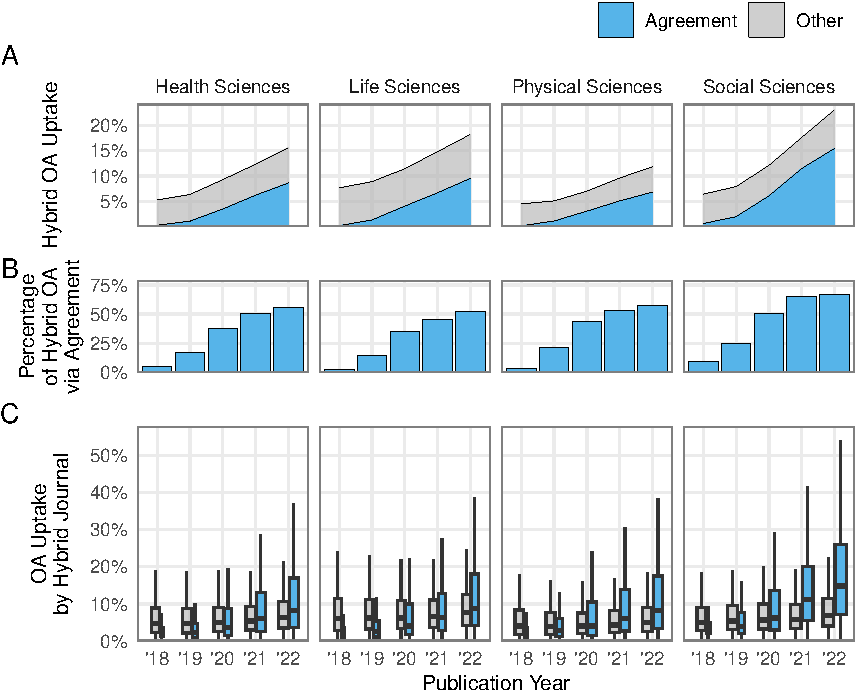
\includegraphics[width=0.99\linewidth,]{fig/subject_panel-1} 

}

\caption{Developement of open access in hybrid journals in transformative agreements between 2018 and 2022 by AJCS subject area. The blue areas represent open access through transformative agreements, the grey areas depict open access articles where no link to an agreement could be established. (A) Proportion of open access articles in hybrid journals per year and publisher. (B) Percentage of hybrid open access via agreements per year and publisher. Boxplots (C) show individual open access uptake rates by individual hybrid journals and open access funding per publication year and publisher. The individual outliers are not shown. Note that data on transformative agreements ending before June 2021 were not available for this study.}\label{fig:subject_panel}
\end{figure}

Figure \ref{fig:subject_panel}C shows that this trend is consistent
across hybrid journals belonging to the ASJC subject area Social
Sciences. In 2022, 25\% of Social Sciences journals provided open access
to at least every fourth article exclusively through transformative
agreements. However, hybrid open access through transformative
agreements played a comparable lesser role in the Life Sciences and
Health Sciences. In these two subject areas, only about half of the open
access articles can be linked to these agreements, both overall and on
median average across journals. In contrast, the majority of Physical
Science Journals, shows an increase of open access through
transformative agreements compared to other options to publish open
access in hybrid journals.

\hypertarget{comparing-countries}{%
\subsection{Comparing countries}\label{comparing-countries}}

Between 2018 and 2022, high-income countries almost exclusively
dominated hybrid open access publishing through transformative
agreements. During this period, first-authors affiliated with
institutions from Organisation for Economic Co-operation and Development
(OECD) member countries published 602,050 open access articles in hybrid
journals, representing 81\% of the investigated open access articles.
This disparity between OECD nations and other countries becomes even
more evident when considering open access through transformative
agreements, as 310,712 of 328,957, or 94\% of open access articles were
associated with such agreements.

Figure \ref{fig:country_patch}A shows the development of hybrid open
access publishing by countries, comparing the OECD area with the BRICS,
an intergovernmental organisation, which comprised the countries Brazil,
Russia, India, China and South Africa as of 2022. The residual category
``Other'' includes the remaining countries. From 2018 to 2022, the
proportion of open access in hybrid journals increased from 6.1\% in
2018 to 26\% in 2022. On the other hand, BRICS recorded an low uptake,
from 1.6\% in 2018 to 3.7\% in 2022.\\
Despite rise of open access across OECD countries, the overall
publication output decreased sharply, dropping to 786,903 in 2022 after
peaking 892,197 articles in 2020. In stark contrast, the number of
articles published in hybrid journals by first authors affiliated with
institutions from BRICS countries increased steadily over the years,
more than doubling from 356,632 in 2018 to 786,903 in 2022. Upon closer
examination, this trend can be observed across all big three publishers,
although the shift towards BRICS is particularly evident in Elsevier's
hybrid journal portfolio, in particular with regard to articles
published in Physical Sciences journals. While OECD publication output
in Elsevier's Physical Sciences journals declined from 112,822 articles
in 2018 to 103,766 in 2022, BRICS output increased from 104,654 to
171,713 in the same five-year period. Furthermore, OECD publication
output in Health Science Journals and Life Science journals stagnated
across the investigated hybrid journal portfolios after a peak in 2020.

\begin{figure}[ht!]

{\centering 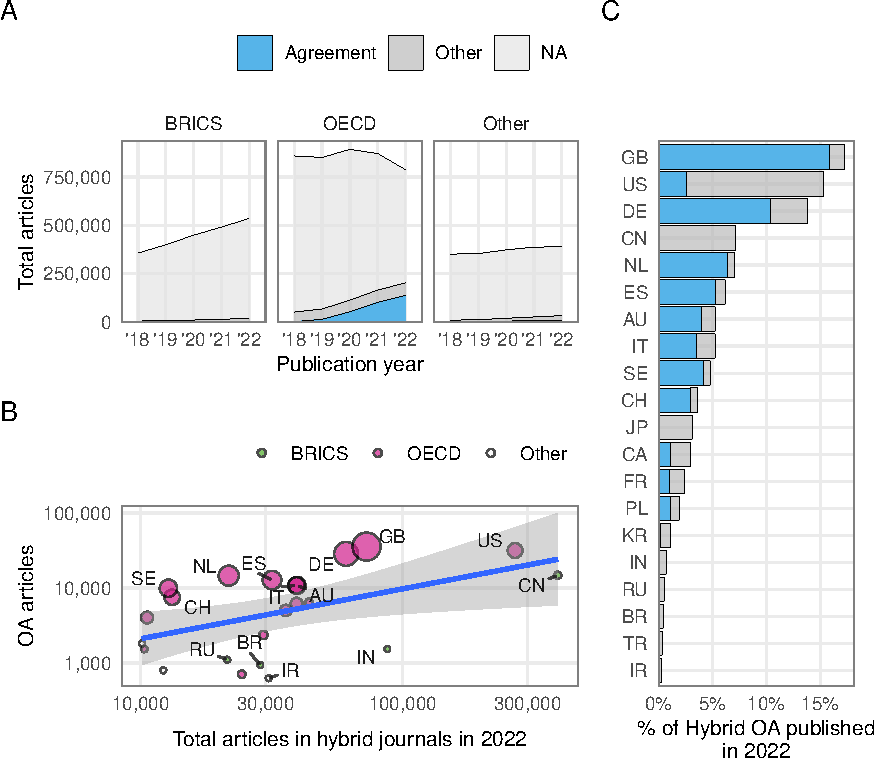
\includegraphics[width=0.99\linewidth,]{fig/country_patch-1} 

}

\caption{Development of hybrid open access publishing by country. (A) presents the number of articles published in hybrid journals included in transformative agreement, distinguishing between BRICS as of 20222, OECD and other countries. (B) Scatterplot contrasting total articles with open access article volume in 2022, by country. Point size represents the number of articles enabled through transformative agreements. (C) Hybrid open access market share in 2022 by country. In (A) and (C), the blue areas represent open access through transformative agreements, the grey areas depict open access articles where no link to an agreement could be established. Country names are represented as ISO two-letter country codes.}\label{fig:country_patch}
\end{figure}

To illustrate the situation in 2022, Figure \ref{fig:country_patch}B
compares total publication output with the number of open access
articles. With 391,530 articles, China was the most productive country,
followed by the United States (268,965 articles) and India (87,428
articles). In contrast, West and Nord European countries published a
considerable high number of open access articles, mainly due to
transformative agreements. Particularly, Germany, Great Britain, the
Netherlands, Sweden, Switzerland and Spain recorded an above-average
open access share as indicated by the linear trend line. As represented
by the point size, as well as it can been seen in Figure
\ref{fig:country_patch}C, transformative agreements contributed to these
market positions. Interestingly, the United States had a notable open
access market share of 15\%, although transformative agreements
contributed to a lesser extent. Similarly, China's open access market
share of 7.2\% in 2022 was comparable to that of the Netherlands, which
was 7.1\%.

Figure \ref{fig:country_top_20_plot} illustrates the development of
hybrid open access from 2018 to 2022, highlighting the top 20 most
productive countries in terms of articles published in hybrid journals
that were included in transformative agreements over the five-year
period. Notably, The Netherlands (27\%), Sweden (24\%), Poland (17\%)
and Great Britain (17\%)) exhibited a relatively high level of uptake in
2018 which continued to increase in the following years. In 2022, Sweden
had the highest proportion of open access relative to its publication
output (78\%), followed by the Netherlands (67\%) and Switzerland
(57\%), with these countries benefiting from transformative agreements.
In Germany, however, hybrid open access only began to increase from 2019
onwards after the successful negotiation of nationwide agreements with
Wiley (July 2019) and Springer Nature (January 2020). Prior to this,
only a few organisations had agreements in place, for the example the
Max Planck Society with Springer Compact.

\begin{figure}[ht!]

{\centering 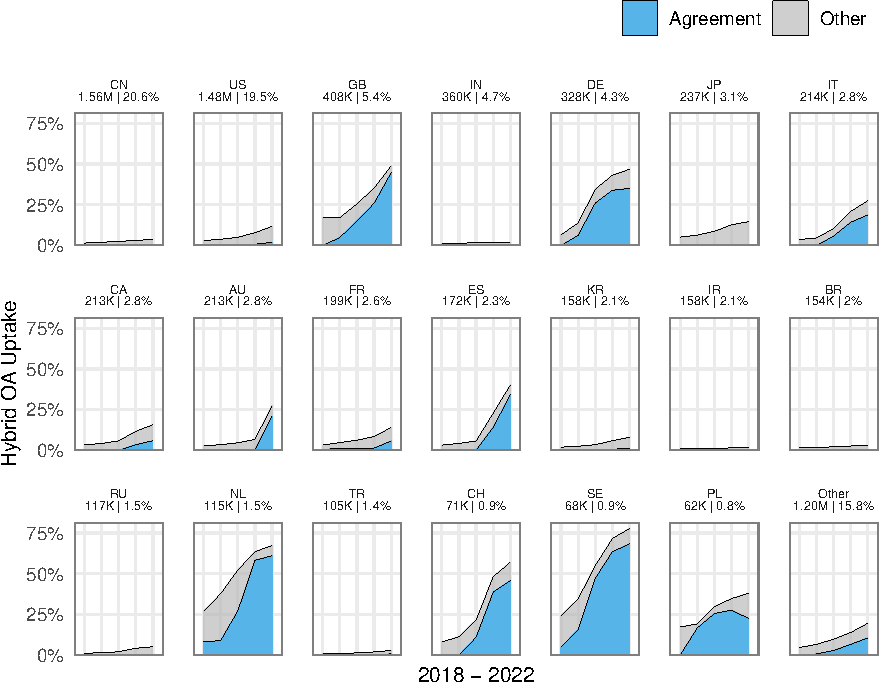
\includegraphics[width=0.99\linewidth,]{fig/country_top_20_plot-1} 

}

\caption{Development of open access in hybrid journals in transformative agreements between 2018 and 2022, by the Top 20 most productive countries in terms of total articles published in the five-years period. Blue areas represent open access through transformative agreements, the grey areas depict open access articles where no link to an agreement could be established. Country names are represented as ISO two-letter country codes}\label{fig:country_top_20_plot}
\end{figure}

Since 2021, there has been a general trend towards hybrid open access
among many high-income countries, primarily driven by transformative
agreements. However, proliferation of transformative agreements differed
across these countries. For instance, Germany successfully negotiated an
agreement with Elsevier not until 2023. Additionally, publication limits
or eligibility criteria for institutions and article types may explain
why even countries with widespread agreement implementation do not
achieve 100\% hybrid open access. Interestingly, in Japan and the US
other options than transformative agreements were the main driver for
the increase in hybrid open access. Once again, the graph highlights
countries with low hybrid open access, particularly non-OECD countries,
where only a few or no agreements were in place.

\hypertarget{discussion}{%
\section{Discussion}\label{discussion}}

The primary aim of this study was to investigate the adoption of open
access in hybrid journals through transformative agreements, presenting
a novel approach based on open data. The results indicate a steady
increase, estimating that the majority of open access in hybrid journals
in 2022 originate from institutions that had an transformative agreement
in place. Yet, the majority of research literature published in hybrid
journals between 2018 and 2022 remained behind a publisher paywall.
Growth in the adoption of open access in hybrid journals through
transformative agreements can be largely attributed to big three
commercial publishers -- Elsevier, Springer Nature, and Wiley -- but
varies across journals, publishers, subjects, and country affiliations.
Despite limitations regarding the data used, the findings indicate that
the current level of implementation of transformative agreements is
insufficient to bring about a large-scale transformation to full open
access.

Presenting an initial overview, some journals recorded substantial open
access uptake rates through transformative agreements. Previous research
indicate that these journals highlight specific areas where publisher
portfolios already had strong market positions {[}@{]}.

\hypertarget{conclusions}{%
\section{Conclusions}\label{conclusions}}

\hypertarget{references}{%
\section*{References}\label{references}}
\addcontentsline{toc}{section}{References}

\hypertarget{refs}{}
\begin{CSLReferences}{1}{0}
\leavevmode\vadjust pre{\hypertarget{ref-Bakker_2024}{}}%
Bakker, C., Langham-Putrow, A., \& Riegelman, A. (2024). Impact of
transformative agreements on publication patterns: An analysis based on
agreements from the ESAC registry. \emph{International Journal of
Librarianship}, \emph{8}(4), 67--96.
\url{https://doi.org/10.23974/ijol.2024.vol8.4.341}

\leavevmode\vadjust pre{\hypertarget{ref-Bergstrom_2014}{}}%
Bergstrom, T. C., Courant, P. N., McAfee, R. P., \& Williams, M. A.
(2014). Evaluating big deal journal bundles. \emph{Proceedings of the
National Academy of Sciences}, \emph{111}(26), 9425--9430.
\url{https://doi.org/10.1073/pnas.1403006111}

\leavevmode\vadjust pre{\hypertarget{ref-Bj_rk_2012}{}}%
Björk, B.-C. (2012). The hybrid model for open access publication of
scholarly articles: A failed experiment? \emph{Journal of the American
Society for Information Science and Technology}, \emph{63}(8),
1496--1504. \url{https://doi.org/10.1002/asi.22709}

\leavevmode\vadjust pre{\hypertarget{ref-Bj_rk_2017}{}}%
Björk, B.-C. (2017). Growth of hybrid open access, 2009--2016.
\emph{PeerJ}, \emph{5}, e3878. \url{https://doi.org/10.7717/peerj.3878}

\leavevmode\vadjust pre{\hypertarget{ref-BJ_RK_2014}{}}%
Björk, B.-C., \& Solomon, D. (2014). How research funders can finance
APCs in full OA and hybrid journals. \emph{Learned Publishing},
\emph{27}(2), 93--103. \url{https://doi.org/10.1087/20140203}

\leavevmode\vadjust pre{\hypertarget{ref-Borrego_2023}{}}%
Borrego, Á. (2023). Article processing charges for open access journal
publishing: A review. \emph{Learned Publishing}, \emph{36}(3), 359--378.
\url{https://doi.org/10.1002/leap.1558}

\leavevmode\vadjust pre{\hypertarget{ref-Borrego_2020}{}}%
Borrego, Á., Anglada, L., \& Abadal, E. (2020). Transformative
agreements: Do they pave the way to open access? \emph{Learned
Publishing}. \url{https://doi.org/10.1002/leap.1347}

\leavevmode\vadjust pre{\hypertarget{ref-Brainard_2023}{}}%
Brainard, J. (2023). {`Transformative'} journals get booted for
switching to open access too slowly. In \emph{Science: SCIENCEINSIDER}.
\url{https://doi.org/10.1126/science.adj3282}

\leavevmode\vadjust pre{\hypertarget{ref-goldoa}{}}%
Bruns, A., Cakir, Y., Kaya, S., \& Beidaghi, S. (2022).
\emph{{ISSN-Matching of Gold OA Journals (ISSN-GOLD-OA) 5.0}}. Bielefeld
University. \url{https://doi.org/10.4119/unibi/2961544}

\leavevmode\vadjust pre{\hypertarget{ref-Butler_2023}{}}%
Butler, L.-A., Matthias, L., Simard, M.-A., Mongeon, P., \& Haustein, S.
(2023). The oligopoly's shift to open access: How the big five academic
publishers profit from article processing charges. \emph{Quantitative
Science Studies}, 1--22. \url{https://doi.org/10.1162/qss_a_00272}

\leavevmode\vadjust pre{\hypertarget{ref-Dallmeier_2010}{}}%
Dallmeier-Tiessen, S., Goerner, B., Darby, R., Hyppoelae, J.,
Igo-Kemenes, P., Kahn, D., Lambert, S., Lengenfelder, A., Leonard, C.,
Mele, S., Polydoratou, P., Ross, D., Ruiz-Perez, S., Schimmer, R.,
Swaisland, M., \& Stelt, W. van der. (2010). \emph{{Open Access
Publishing - Models and Attributes}} (T. S. consortium, Ed.).

\leavevmode\vadjust pre{\hypertarget{ref-Fraser_2023}{}}%
Fraser, N., Hobert, A., Jahn, N., Mayr, P., \& Peters, I. (2023). No
deal: German researchers' publishing and citing behaviors after big deal
negotiations with elsevier. \emph{Quantitative Science Studies},
\emph{4}(2), 325--352. \url{https://doi.org/10.1162/qss_a_00255}

\leavevmode\vadjust pre{\hypertarget{ref-Geschuhn_2017}{}}%
Geschuhn, K., \& Stone, G. (2017). It's the workflows, stupid! What is
required to make {`offsetting'} work for the open access transition.
\emph{Insights the {UKSG} Journal}, \emph{30}(3), 103--114.
\url{https://doi.org/10.1629/uksg.391}

\leavevmode\vadjust pre{\hypertarget{ref-Haucap_2021}{}}%
Haucap, J., Moshgbar, N., \& Schmal, W. B. (2021). The impact of the
german {``DEAL''} on competition in the academic publishing market.
\emph{Managerial and Decision Economics}, \emph{42}(8), 2027--2049.
\url{https://doi.org/10.1002/mde.3493}

\leavevmode\vadjust pre{\hypertarget{ref-Hinchliffe_2019}{}}%
Hinchliffe, L. J. (2019). \emph{Transformative agreements: A primer}.
\url{https://web.archive.org/web/20210128170342/https://scholarlykitchen.sspnet.org/2019/04/23/transformative-agreements/};
The Scholarly Kitchen.

\leavevmode\vadjust pre{\hypertarget{ref-Huang_2020}{}}%
Huang, C.-K. (Karl), Neylon, C., Hosking, R., Montgomery, L., Wilson, K.
S., Ozaygen, A., \& Brookes-Kenworthy, C. (2020). Evaluating the impact
of open access policies on research institutions. \emph{{eLife}},
\emph{9}. \url{https://doi.org/10.7554/elife.57067}

\leavevmode\vadjust pre{\hypertarget{ref-jahn2023}{}}%
Jahn, N., Haupka, N., \& Hobert, A. (2023). \emph{Analysing and
reclassifying open access information in OpenAlex}. Blog post.
\url{https://subugoe.github.io/scholcomm_analytics/posts/oalex_oa_status/}

\leavevmode\vadjust pre{\hypertarget{ref-Jahn_2021}{}}%
Jahn, N., Matthias, L., \& Laakso, M. (2022). Toward transparency of
hybrid open access through publisher-provided metadata: An article-level
study of elsevier. \emph{Journal of the Association for Information
Science and Technology}, \emph{73}(1), 104--118.
\url{https://doi.org/10.1002/asi.24549}

\leavevmode\vadjust pre{\hypertarget{ref-Jahn_2016}{}}%
Jahn, N., \& Tullney, M. (2016). A study of institutional spending on
open access publication fees in germany. \emph{{PeerJ}}, \emph{4},
e2323. \url{https://doi.org/10.7717/peerj.2323}

\leavevmode\vadjust pre{\hypertarget{ref-Jubb_2017}{}}%
Jubb, M., Plume, A., Oeben, S., Brammer, L., Johnson, R., Bütün, C., \&
Pinfield, S. (2017). \emph{Monitoring the transition to open access:
December 2017}.
\url{https://web.archive.org/web/20200212015524/https://www.universitiesuk.ac.uk/policy-and-analysis/reports/Documents/2017/monitoring-transition-open-access-2017.pdf}

\leavevmode\vadjust pre{\hypertarget{ref-Laakso_2016}{}}%
Laakso, M., \& Björk, B.-C. (2016). Hybrid open access--a longitudinal
study. \emph{Journal of Informetrics}, \emph{10}(4), 919--932.
\url{https://doi.org/10.1016/j.joi.2016.08.002}

\leavevmode\vadjust pre{\hypertarget{ref-Larivi_re_2016}{}}%
Larivière, V., Desrochers, N., Macaluso, B., Mongeon, P., Paul-Hus, A.,
\& Sugimoto, C. R. (2016). Contributorship and division of labor in
knowledge production. \emph{Social Studies of Science}, \emph{46}(3),
417--435. \url{https://doi.org/10.1177/0306312716650046}

\leavevmode\vadjust pre{\hypertarget{ref-Larivi_re_2015}{}}%
Larivière, V., Haustein, S., \& Mongeon, P. (2015). The oligopoly of
academic publishers in the digital era. \emph{{PLOS} {ONE}},
\emph{10}(6), e0127502.
\url{https://doi.org/10.1371/journal.pone.0127502}

\leavevmode\vadjust pre{\hypertarget{ref-Liverpool_2023}{}}%
Liverpool, L. (2023). Open-access reformers launch next bold publishing
plan. \emph{Nature}, \emph{623}(7986), 238--240.
\url{https://doi.org/10.1038/d41586-023-03342-6}

\leavevmode\vadjust pre{\hypertarget{ref-Marques_2020}{}}%
Marques, M., \& Stone, G. (2020). Transitioning to open access: An
evaluation of the {UK} springer compact agreement pilot 2016--2018.
\emph{College {\&} Research Libraries}, \emph{81}(6), 913--927.
\url{https://doi.org/10.5860/crl.81.6.913}

\leavevmode\vadjust pre{\hypertarget{ref-Marques_2019}{}}%
Marques, M., Woutersen-Windhouwer, S., \& Tuuliniemi, A. (2019).
Monitoring agreements with open access elements: Why article-level
metadata are important. \emph{Insights the {UKSG} Journal}, \emph{32}.
\url{https://doi.org/10.1629/uksg.489}

\leavevmode\vadjust pre{\hypertarget{ref-Mart_n_Mart_n_2018}{}}%
Martín-Martín, A., Costas, R., Leeuwen, T. van, \& López-Cózar, E. D.
(2018). Evidence of open access of scientific publications in google
scholar: A large-scale analysis. \emph{Journal of Informetrics},
\emph{12}(3), 819--841. \url{https://doi.org/10.1016/j.joi.2018.06.012}

\leavevmode\vadjust pre{\hypertarget{ref-Marwick_2018}{}}%
Marwick, B., Boettiger, C., \& Mullen, L. (2018). Packaging data
analytical work reproducibly using r (and friends). \emph{The American
Statistician}, \emph{72}(1), 80--88.
\url{https://doi.org/10.1080/00031305.2017.1375986}

\leavevmode\vadjust pre{\hypertarget{ref-Matthias_2019}{}}%
Matthias, L., Jahn, N., \& Laakso, M. (2019). The two-way street of open
access journal publishing: Flip it and reverse it. \emph{Publications},
\emph{7}(2), 23. \url{https://doi.org/10.3390/publications7020023}

\leavevmode\vadjust pre{\hypertarget{ref-Mittermaier_2021}{}}%
Mittermaier, B. (2021). {Rolle des Open Access Monitor Deutschland bei
der Antragstellung im DFG-Förderprogramm
Open-Access-Publikationskosten}. \emph{{O-Bib. Das Offene
Bibliotheksjournal / Herausgeber VDB}}, \emph{8}.
\url{https://doi.org/10.5282/O-BIB/5731}

\leavevmode\vadjust pre{\hypertarget{ref-Momeni_2023}{}}%
Momeni, F., Dietze, S., Mayr, P., Biesenbender, K., \& Peters, I.
(2023). Which factors are associated with open access publishing? A
springer nature case study. \emph{Quantitative Science Studies},
\emph{4}(2), 353--371. \url{https://doi.org/10.1162/qss_a_00253}

\leavevmode\vadjust pre{\hypertarget{ref-Momeni_2021}{}}%
Momeni, F., Mayr, P., Fraser, N., \& Peters, I. (2021). What happens
when a journal converts to open access? A bibliometric analysis.
\emph{Scientometrics}, \emph{126}(12), 9811--9827.
\url{https://doi.org/10.1007/s11192-021-03972-5}

\leavevmode\vadjust pre{\hypertarget{ref-Moskovkin_2022}{}}%
Moskovkin, V. M., Saprykina, T. V., \& Boichuk, I. V. (2022).
Transformative agreements in the development of open access.
\emph{Journal of Electronic Resources Librarianship}, \emph{34}(3),
165--207. \url{https://doi.org/10.1080/1941126x.2022.2099000}

\leavevmode\vadjust pre{\hypertarget{ref-Parmhed_2023}{}}%
Parmhed, S., \& Säll, J. (2023). Transformative agreements and their
practical impact: A librarian perspective. \emph{Insights the UKSG
Journal}, \emph{36}. \url{https://doi.org/10.1629/uksg.612}

\leavevmode\vadjust pre{\hypertarget{ref-Pieper_2018}{}}%
Pieper, D., \& Broschinski, C. (2018). {OpenAPC}: A contribution to a
transparent and reproducible monitoring of fee-based open access
publishing across institutions and nations. \emph{Insights the {UKSG}
Journal}, \emph{31}. \url{https://doi.org/10.1629/uksg.439}

\leavevmode\vadjust pre{\hypertarget{ref-Pinfield_2016}{}}%
Pinfield, S., Salter, J., \& Bath, P. A. (2016). The "total cost of
publication" in a hybrid open-access environment: Institutional
approaches to funding journal article-processing charges in combination
with subscriptions. \emph{Journal of the Association for Information
Science and Technology}, \emph{67}(7), 1751--1766.
\url{https://doi.org/10.1002/asi.23446}

\leavevmode\vadjust pre{\hypertarget{ref-Pinhasi_2021}{}}%
Pinhasi, R., Hölbling, L., \& Kromp, B. (2021). Austrian transition to
open access: A collaborative approach. \emph{Insights the UKSG Journal},
\emph{34}. \url{https://doi.org/10.1629/uksg.561}

\leavevmode\vadjust pre{\hypertarget{ref-Pinhasi_2020}{}}%
Pinhasi, R., Kromp, B., Blechl, G., \& Hölbling, L. (2020). The impact
of open access publishing agreements at the {University of Vienna} in
light of the plan s requirements: A review of current status, challenges
and perspectives. \emph{Insights the UKSG Journal}, \emph{33}.
\url{https://doi.org/10.1629/uksg.523}

\leavevmode\vadjust pre{\hypertarget{ref-Piwowar_2018}{}}%
Piwowar, H., Priem, J., Larivière, V., Alperin, J. P., Matthias, L.,
Norlander, B., Farley, A., West, J., \& Haustein, S. (2018). The state
of {OA}: A large-scale analysis of the prevalence and impact of open
access articles. \emph{{PeerJ}}, \emph{6}, e4375.
\url{https://doi.org/10.7717/peerj.4375}

\leavevmode\vadjust pre{\hypertarget{ref-P_l_nen_2020}{}}%
Pölönen, J., Laakso, M., Guns, R., Kulczycki, E., \& Sivertsen, G.
(2020). Open access at the national level: A comprehensive analysis of
publications by finnish researchers. \emph{Quantitative Science
Studies}, \emph{1}(4), 1396--1428.
\url{https://doi.org/10.1162/qss_a_00084}

\leavevmode\vadjust pre{\hypertarget{ref-priem2022openalex}{}}%
Priem, J., Piwowar, H., \& Orr, R. (2022). \emph{OpenAlex: A fully-open
index of scholarly works, authors, venues, institutions, and concepts}.
\url{https://arxiv.org/abs/2205.01833}

\leavevmode\vadjust pre{\hypertarget{ref-Prosser_2003}{}}%
Prosser, D. C. (2003). From here to there: A proposed mechanism for
transforming journals from closed to open access. \emph{Learned
Publishing}, \emph{16}(3), 163--166.
\url{https://doi.org/10.1087/095315103322110923}

\leavevmode\vadjust pre{\hypertarget{ref-Goodin_2023}{}}%
Rasmussen, K. B. (2023). Interview with {Robert {`Bob'} E. Goodin}.
\emph{Tidskrift För Politisk Filosofi}.
\url{https://www.politiskfilosofi.se/fulltext/2023-2/pdf/TPF_2023-2_interview_with_robert_bob_e_goodin.pdf}

\leavevmode\vadjust pre{\hypertarget{ref-Robinson_Garcia_2020}{}}%
Robinson-Garcia, N., Costas, R., \& Leeuwen, T. N. van. (2020). Open
access uptake by universities worldwide. \emph{{PeerJ}}, \emph{8},
e9410. \url{https://doi.org/10.7717/peerj.9410}

\leavevmode\vadjust pre{\hypertarget{ref-Schiltz_2018}{}}%
Schiltz, M. (2018). Science without publication paywalls: cOAlition s
for the realisation of full and immediate open access. \emph{PLOS
Biology}, \emph{16}(9), e3000031.
\url{https://doi.org/10.1371/journal.pbio.3000031}

\leavevmode\vadjust pre{\hypertarget{ref-Schimmer_2015}{}}%
Schimmer, R., Geschuhn, K., \& Vogler, A. (2015). \emph{{Disrupting the
subscription journals'business model for the necessary large-scale
transformation to open access}}. Max Planck Digital Library.
\url{https://doi.org/10.17617/1.3}

\leavevmode\vadjust pre{\hypertarget{ref-Shu_2023}{}}%
Shu, F., \& Larivière, V. (2023). The oligopoly of open access
publishing. \emph{Scientometrics}, \emph{129}(1), 519--536.
\url{https://doi.org/10.1007/s11192-023-04876-2}

\leavevmode\vadjust pre{\hypertarget{ref-Taubert_2023}{}}%
Taubert, N., Hobert, A., Jahn, N., Bruns, A., \& Iravani, E. (2023).
Understanding differences of the OA uptake within the german university
landscape (2010--2020): Part 1---journal-based OA.
\emph{Scientometrics}, \emph{128}(6), 3601--3625.
\url{https://doi.org/10.1007/s11192-023-04716-3}

\leavevmode\vadjust pre{\hypertarget{ref-Wenaas_2022}{}}%
Wenaas, L. (2022). Choices of immediate open access and the relationship
to journal ranking and publish-and-read deals. \emph{Frontiers in
Research Metrics and Analytics}, \emph{7}.
\url{https://doi.org/10.3389/frma.2022.943932}

\leavevmode\vadjust pre{\hypertarget{ref-Zhang_2022}{}}%
Zhang, L., Wei, Y., Huang, Y., \& Sivertsen, G. (2022). Should open
access lead to closed research? The trends towards paying to perform
research. \emph{Scientometrics}, \emph{127}(12), 7653--7679.
\url{https://doi.org/10.1007/s11192-022-04407-5}

\end{CSLReferences}

\end{document}